% =============================================================================
% CHƯƠNG 3: THIẾT KẾ MÔ HÌNH MẠNG
% =============================================================================
\chapter{Thiết kế mô hình mạng}

\section{Tổng quan thiết kế}

Mô hình mạng được thiết kế gồm hai phần chính:
\begin{enumerate}
    \item \textbf{Mạng nội bộ (LAN) tại 3 chi nhánh}: Mỗi chi nhánh dùng một kiến trúc LAN khác nhau để so sánh hiệu năng.
    \item \textbf{Backbone Metro Ethernet MPLS của ISP}: Các router CE, PE, P tạo thành hạ tầng kết nối xuyên chi nhánh.
\end{enumerate}

\begin{figure}[H]
    \centering
    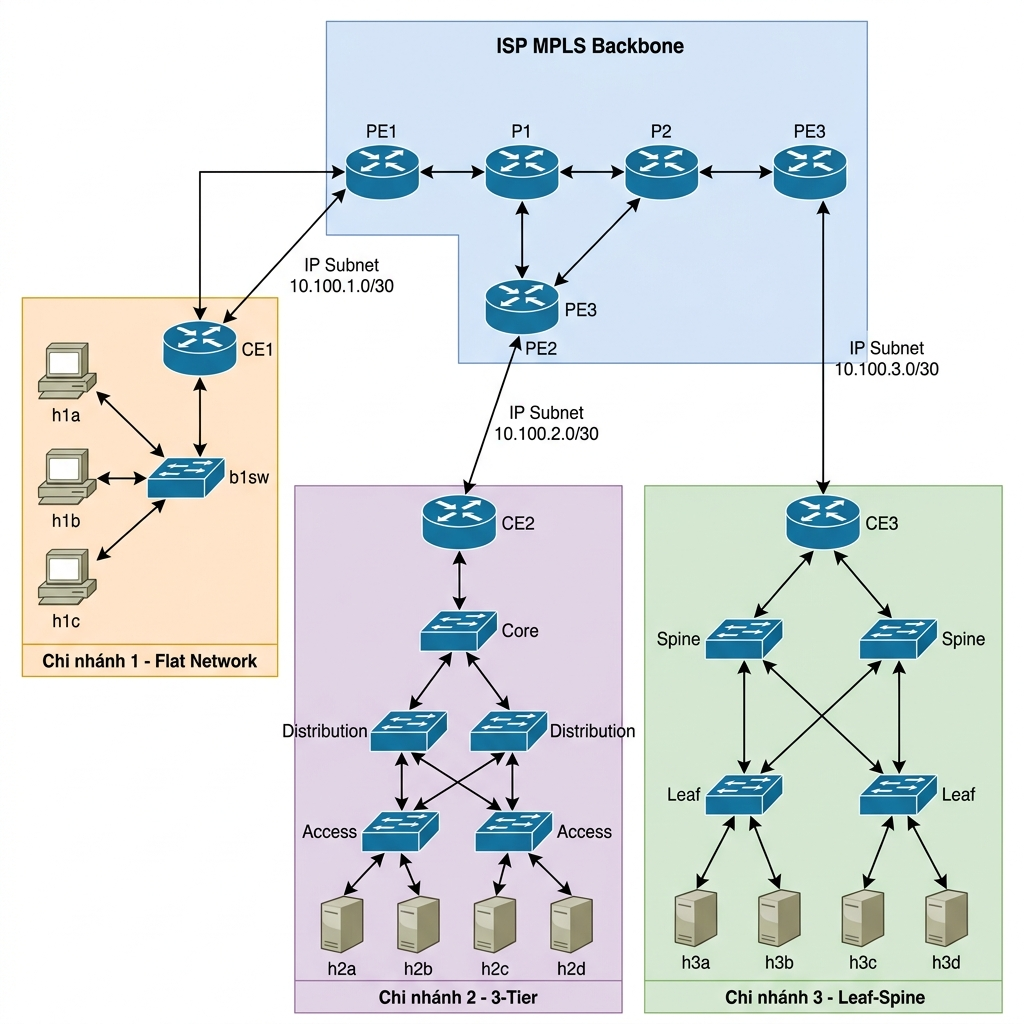
\includegraphics[width=0.95\linewidth]{media/mpls_topology.png}
    \caption{Sơ đồ tổng thể mô hình Metro Ethernet MPLS kết nối 3 chi nhánh}
    \label{fig:mpls_topology}
\end{figure}

\subsection{Sơ đồ logic tổng thể}

\begin{figure}[H]
    \centering
    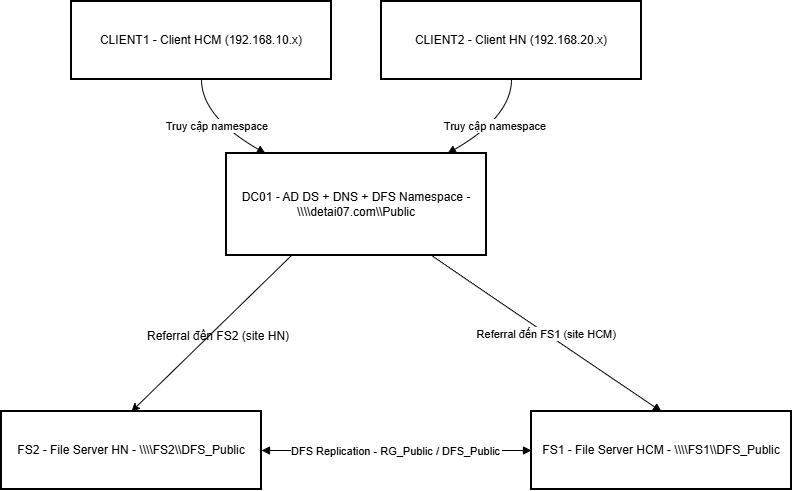
\includegraphics[width=0.85\linewidth]{media/so_do_kien_truc.png}
    \caption{Sơ đồ kiến trúc tổng thể hệ thống}
    \label{fig:kientruc}
\end{figure}

Cấu trúc logic tổng thể hệ thống được mô tả nhằm sau:

\begin{Verbatim}[fontsize=\small, frame=single]
+----------------------------------------------------------+
|           ISP METRO ETHERNET MPLS BACKBONE               |
|                                                          |
|  +-----+  10.10.11.0/30  +----+  10.20.12.0/30  +-----+ |
|  | PE1 |---------------->| P1 |<--------------->| P2  | |
|  +-----+                 +-+--+                 +--+--+ |
|     |                      |  10.20.13.0/30        |    |
|     |                   +--+--+           +----+---+    |
|     |       10.20.13    | P3  |    10.20.24    | P4 |   |
|     |                   +--+--+           +----+---+    |
|     |                      |10.10.23.0/30      |         |
|     |                   +--v--+           +----|---+    |
|     |                   | PE2 |           |  PE3   |    |
+-----|-------------------+-----+-----------+--------+----+
      |10.0.1.0/30        |10.0.2.0/30     |10.0.3.0/30
   +--v--+            +---v--+          +---v--+
   | CE1 |            | CE2  |          | CE3  |
   +--+--+            +--+---+          +--+---+
      |                  |                 |
+-----v------+   +-------v------+   +------v------+
| Branch 1   |   | Branch 2     |   | Branch 3    |
| Flat Net   |   | 3-Tier CDA   |   | Leaf-Spine  |
| host1-4    |   | admin,lab,   |   | web,dns,db  |
| 10.1.0.0/24|   | guest hosts  |   | servers     |
+------------+   +--------------+   +-------------+
\end{Verbatim}



\section{Thiết kế chi nhánh 1: Mạng phẳng (Flat Network)}

\subsection{Cấu trúc topology}

Chi nhánh 1 sử dụng kiến trúc mạng phẳng đơn giản nhất:

\begin{Verbatim}[fontsize=\small, frame=single]
   CE1 (gateway: 10.1.0.1/24)
    |
   [s_acc1 - Access Switch Layer 2]
    |---------|---------|---------
  host1     host2    host3   host4
10.1.0.101 10.1.0.102 10.1.0.103 10.1.0.104
\end{Verbatim}

\textbf{Mô tả:}
\begin{itemize}
    \item 1 switch Layer 2 duy nhất (s\_acc1) kết nối tất cả host.
    \item 4 host: host1, host2, host3, host4 -- cùng subnet 10.1.0.0/24.
    \item CE1\_lan đóng vai trò default gateway và kết nối lên PE1.
    \item Không có VLAN, không có routing nội bộ.
\end{itemize}

\subsection{Thông số kỹ thuật}
\begin{itemize}
    \item Số switch: 1 (OVS, failMode=standalone)
    \item Số host: 4 (host1, host2, host3, host4)
    \item Băng thông host-switch: không giới hạn (virtual link)
    \item Subnet: 10.1.0.0/24, Gateway: 10.1.0.1
\end{itemize}

\section{Thiết kế chi nhánh 2: Mạng 3 lớp (Core--Distribution--Access)}

\subsection{Cấu trúc topology}

\begin{Verbatim}[fontsize=\small, frame=single]
         CE2_LAN (Inter-VLAN Router)
          |------------|
        core1        core2
          |-----|    |-----|
         dist1       dist2
          /---\ \    / /---\
        acc1  acc2  acc2  acc3
         |     |         |
     admin1  lab1-2   guest1-2
     admin2
VLAN10: admin (10.2.10.0/24)
VLAN20: lab   (10.2.20.0/24)
VLAN30: guest (10.2.30.0/24)
\end{Verbatim}

\textbf{Mô tả:}
\begin{itemize}
    \item \textbf{Access switches} (acc1, acc2, acc3): Kết nối host, mỗi switch 2 host.
    \item \textbf{Distribution switches} (dist1, dist2): Tập hợp uplink từ access, cross-connected để dự phòng.
    \item \textbf{Core switches} (core1, core2): Kết nối distribution lên CE2\_lan (dual uplink).
    \item CE2\_lan: Inter-VLAN routing giữa 3 VLAN (Admin/Lab/Guest) + kết nối lên PE2.
\end{itemize}

\subsection{Thông số kỹ thuật}
\begin{itemize}
    \item Số switch: 7 (Core x2 + Dist x2 + Access x3)
    \item Số host: 6 (admin1-2, lab1-2, guest1-2)
    \item VLAN10=10.2.10.0/24, VLAN20=10.2.20.0/24, VLAN30=10.2.30.0/24
    \item Link Core--CE2\_lan: dual uplink (10.2.0.0/30 và 10.2.0.4/30)
\end{itemize}

\section{Thiết kế chi nhánh 3: Mạng Leaf-Spine}

\subsection{Cấu trúc topology}

\begin{Verbatim}[fontsize=\small, frame=single]
    CE3_LAN (gateway + dual uplink)
     |------------|
  [spine1]------[spine2]    <- Spine (loi, full-mesh)
   / | \        / | \
 lf1  lf2  lf3 lf1 lf2 lf3  <- Leaf (truy cap, moi leaf noi ca 2 spine)
  |    |    |
 web  dns   db               <- Server zones
 1-2  1-2   1-2

Web zone : 10.3.10.0/24
DNS zone : 10.3.20.0/24
DB  zone : 10.3.30.0/24
\end{Verbatim}

\textbf{Mô tả:}
\begin{itemize}
    \item 2 \textbf{Spine} switch (spine1, spine2): Lõi băng thông cao, kết nối full-mesh với mỗi Leaf.
    \item 3 \textbf{Leaf} switch (leaf1, leaf2, leaf3): Truy cập server, mỗi Leaf kết nối cả 2 Spine.
    \item Full Mesh Spine-Leaf cho phép ECMP (Equal-Cost Multi-Path).
    \item CE3\_lan kết nối cả hai Spine để tăng dự phòng.
\end{itemize}

\subsection{Thông số kỹ thuật}
\begin{itemize}
    \item Số switch: 5 (Spine x2 + Leaf x3)
    \item Số host: 6 (web1-2, dns1-2, db1-2)
    \item Mỗi Leaf có 2 uplink lên Spine (redundant path)
    \item CE3\_lan: dual uplink lên spine1 (10.3.0.0/30) và spine2 (10.3.0.4/30)
\end{itemize}

\section{Thiết kế backbone MPLS của ISP}

\subsection{Topology backbone}

\begin{Verbatim}[fontsize=\small, frame=single]
Backbone MPLS (4P + 3PE):

PE1 ---[10.10.11.0/30]--- P1 ---[10.20.12.0/30]--- P2 ---[10.10.32.0/30]--- PE3
         |                 |                          |
         |     [10.20.13]  |      [10.20.23]          |
         |                 P3 --[10.10.23.0/30]-- PE2
         |                 |
         |     [10.20.14/10.20.24/10.20.34]
         |                 P4
         +--[10.10.13.0/30]--+--[10.10.24.0/30]--PE2
                              +--[10.10.34.0/30]--PE3
\end{Verbatim}

\textbf{Mô tả thiết bị:}
\begin{itemize}
    \item \textbf{PE1}: Kết nối CE1 (chi nhánh 1). Push label khi gói vào, nhận label khi gói ra.
    \item \textbf{PE2}: Kết nối CE2 (chi nhánh 2). Dual uplink lên P3 và P4.
    \item \textbf{PE3}: Kết nối CE3 (chi nhánh 3). Dual uplink lên P2 và P4.
    \item \textbf{P1, P2, P3, P4}: Provider Core -- chỉ Swap label, kết nối full-mesh với nhau.
\end{itemize}

\subsection{Kế hoạch nhãn MPLS (Label Plan)}

\begin{table}[H]
    \centering
    \caption{Bảng phân phối nhãn MPLS (LFIB -- Label Forwarding Information Base)}
    \vspace{0.3cm}
    \small
    \begin{tabularx}{\textwidth}{|c|c|>{\raggedright\arraybackslash}X|c|c|}
        \hline
        \textbf{Node} & \textbf{Thao tác} & \textbf{Mục tiêu} & \textbf{Label vào} & \textbf{Label ra} \\ \hline
        PE1 & PUSH & 10.2.0.0/16 (LAN2) via P1 & -- & 200 \\ \hline
        PE1 & PUSH & 10.3.0.0/16 (LAN3) via P1 & -- & 300 \\ \hline
        PE2 & PUSH & 10.1.0.0/24 (LAN1) via P3 & -- & 100 \\ \hline
        PE2 & PUSH & 10.3.0.0/16 (LAN3) via P4 & -- & 310 \\ \hline
        PE3 & PUSH & 10.1.0.0/24 (LAN1) via P2 & -- & 110 \\ \hline
        PE3 & PUSH & 10.2.0.0/16 (LAN2) via P2 & -- & 210 \\ \hline
        P1  & SWAP & forward sang P3 (LAN1$\to$LAN2) & 200 & 201 \\ \hline
        P1  & SWAP & forward sang P2 (LAN1$\to$LAN3) & 300 & 301 \\ \hline
        P2  & SWAP & forward sang P1 (LAN3$\to$LAN1) & 110 & 111 \\ \hline
        P2  & SWAP & forward sang P4 (LAN3$\to$LAN2) & 210 & 211 \\ \hline
        P3  & SWAP & forward sang P1 (LAN2$\to$LAN1) & 100 & 101 \\ \hline
        P3  & SWAP & forward sang P4 (LAN2$\to$LAN3) & 310 & 311 \\ \hline
        P1  & POP  & giao về PE1 (label=0) & 101,111 & 0 \\ \hline
        P3  & POP  & giao về PE2 (label=0) & 201 & 0 \\ \hline
        P2  & POP  & giao về PE3 (label=0) & 301 & 0 \\ \hline
        P4  & POP  & giao về PE2/PE3 & 211,311 & 0 \\ \hline
    \end{tabularx}
    \label{tab:labelplan}
\end{table}

\section{Bảng địa chỉ IP toàn hệ thống}

\begin{table}[H]
    \centering
    \caption{Bảng địa chỉ IP -- LAN chi nhánh}
    \vspace{0.3cm}
    \small
    \begin{tabularx}{\textwidth}{|c|c|c|c|c|}
        \hline
        \textbf{Chi nhánh} & \textbf{Host} & \textbf{Địa chỉ IP} & \textbf{Subnet} & \textbf{Default GW} \\ \hline
        \multirow{5}{*}{1 -- Flat} & host1 & 10.1.0.101 & /24 & 10.1.0.1 \\ \cline{2-5}
                                    & host2 & 10.1.0.102 & /24 & 10.1.0.1 \\ \cline{2-5}
                                    & host3 & 10.1.0.103 & /24 & 10.1.0.1 \\ \cline{2-5}
                                    & host4 & 10.1.0.104 & /24 & 10.1.0.1 \\ \cline{2-5}
                                    & CE1\_lan & 10.1.0.1 & /24 & -- \\ \hline
        \multirow{7}{*}{2 -- 3-Tier} & admin1 & 10.2.10.11 & /24 & 10.2.10.1 \\ \cline{2-5}
                                      & admin2 & 10.2.10.12 & /24 & 10.2.10.1 \\ \cline{2-5}
                                      & lab1   & 10.2.20.21 & /24 & 10.2.20.1 \\ \cline{2-5}
                                      & lab2   & 10.2.20.22 & /24 & 10.2.20.1 \\ \cline{2-5}
                                      & guest1 & 10.2.30.31 & /24 & 10.2.30.1 \\ \cline{2-5}
                                      & guest2 & 10.2.30.32 & /24 & 10.2.30.1 \\ \cline{2-5}
                                      & CE2\_lan-gw & 10.2.x.1 & /24 & -- \\ \hline
        \multirow{7}{*}{3 -- Leaf-Spine} & web1 & 10.3.10.11 & /24 & 10.3.10.1 \\ \cline{2-5}
                                          & web2 & 10.3.10.12 & /24 & 10.3.10.1 \\ \cline{2-5}
                                          & dns1 & 10.3.20.21 & /24 & 10.3.20.1 \\ \cline{2-5}
                                          & dns2 & 10.3.20.22 & /24 & 10.3.20.1 \\ \cline{2-5}
                                          & db1  & 10.3.30.31 & /24 & 10.3.30.1 \\ \cline{2-5}
                                          & db2  & 10.3.30.32 & /24 & 10.3.30.1 \\ \cline{2-5}
                                          & CE3\_lan-gw & 10.3.x.1 & /24 & -- \\ \hline
    \end{tabularx}
    \label{tab:ip_lan}
\end{table}

\begin{table}[H]
    \centering
    \caption{Bảng địa chỉ IP -- Backbone ISP MPLS}
    \vspace{0.3cm}
    \small
    \begin{tabularx}{\textwidth}{|c|c|c|c|}
        \hline
        \textbf{Segment} & \textbf{Router A} & \textbf{Router B} & \textbf{Subnet} \\ \hline
        CE1 -- PE1 & ce1-eth0: 10.0.1.1 & pe1-eth0: 10.0.1.2 & /30 \\ \hline
        CE2 -- PE2 & ce2-eth0: 10.0.2.1 & pe2-eth0: 10.0.2.2 & /30 \\ \hline
        CE3 -- PE3 & ce3-eth0: 10.0.3.1 & pe3-eth0: 10.0.3.2 & /30 \\ \hline
        CE1 -- CE1\_lan & ce1-eth1: 10.100.1.1 & ce1\_lan-eth1: 10.100.1.2 & /30 \\ \hline
        CE2 -- CE2\_lan & ce2-eth1: 10.100.2.1 & ce2\_lan-eth2: 10.100.2.2 & /30 \\ \hline
        CE3 -- CE3\_lan & ce3-eth1: 10.100.3.1 & ce3\_lan-eth2: 10.100.3.2 & /30 \\ \hline
        PE1 -- P1 & pe1-eth1: 10.10.11.1 & p1-eth0: 10.10.11.2 & /30 \\ \hline
        PE1 -- P3 & pe1-eth2: 10.10.13.1 & p3-eth0: 10.10.13.2 & /30 \\ \hline
        PE2 -- P3 & pe2-eth1: 10.10.23.1 & p3-eth1: 10.10.23.2 & /30 \\ \hline
        PE2 -- P4 & pe2-eth2: 10.10.24.1 & p4-eth0: 10.10.24.2 & /30 \\ \hline
        PE3 -- P2 & pe3-eth1: 10.10.32.1 & p2-eth0: 10.10.32.2 & /30 \\ \hline
        PE3 -- P4 & pe3-eth2: 10.10.34.1 & p4-eth1: 10.10.34.2 & /30 \\ \hline
        P1 -- P2 & p1-eth1: 10.20.12.1 & p2-eth1: 10.20.12.2 & /30 \\ \hline
        P1 -- P3 & p1-eth2: 10.20.13.1 & p3-eth2: 10.20.13.2 & /30 \\ \hline
        P1 -- P4 & p1-eth3: 10.20.14.1 & p4-eth2: 10.20.14.2 & /30 \\ \hline
        P2 -- P3 & p2-eth2: 10.20.23.1 & p3-eth3: 10.20.23.2 & /30 \\ \hline
        P2 -- P4 & p2-eth3: 10.20.24.1 & p4-eth3: 10.20.24.2 & /30 \\ \hline
        P3 -- P4 & p3-eth4: 10.20.34.1 & p4-eth4: 10.20.34.2 & /30 \\ \hline
    \end{tabularx}
    \label{tab:ip_backbone}
\end{table}
